\section{Task 4: two storms, one word}\label{sec:q4}

\subsection{Event windows and indices}

We compare the Zhengzhou storm (17--23 July 2021) with the Shanxi storm (1--7 October 2021). For Shanxi we use Taiyuan, which lies in the core of the rain belt, and Yuncheng plus the attachment station 53975099999, which lie on its southern margin; provincial aggregates come from the official reports. Six indices describe each event: total rainfall, one-day maximum, three-day maximum, the longest run of consecutive wet days, the ratio of one-day to three-day rainfall (a concentration measure), and the percentile of that ratio within the station's own climatology. Return periods are computed from the station's 1961--2020 GEV fit.

\begin{table}[H]
\centering
\caption{Event indices. Return periods are GEV estimates; the percentile of the concentration ratio is computed from each station's own annual records.}
\label{tab:q4event}
\small
\begin{tabular}{lrrrrrr}
\toprule
 & Total & 1-day max & 3-day max & Wet run & 1d/3d & RP(1d)\\
 & (mm) & (mm) & (mm) & (days) & ratio & (years)\\
\midrule
Zhengzhou & 362.2 & 188.7 & 313.4 & 5 & 0.60 & 134.5\\
Taiyuan & 203.2 & 85.6 & 182.9 & 5 & 0.47 & 9.5\\
Yuncheng & 52.6 & 18.3 & 39.9 & 4 & 0.46 & 1.0\\
Station 53975 & 26.9 & 10.9 & 20.8 & 4 & 0.52 & 1.0\\
\bottomrule
\end{tabular}
\end{table}

The two core stations differ by a factor of 14 in the rarity of their daily rainfall (134.5 versus 9.5 years) but agree in duration (five consecutive wet days). Zhengzhou's daily total contains 60\% of its three-day total, Taiyuan's only 47\%, and Taiyuan's concentration ratio sits at the 6.5th percentile of its own climatology, i.e.\ the storm was unusually \emph{even} for that station. The southern stations received an order of magnitude less rain, confirming that the October event was concentrated in a narrow belt along the Taihang mountains rather than spread over the province.

\subsection{Are they the same type?}

We formalise the comparison with three criteria, each scaled to be dimensionless:

\begin{enumerate}[leftmargin=1.4em,itemsep=1pt]
\item \emph{Rarity ratio}: $\mathrm{RP}_{1d}(\text{Zhengzhou})/\mathrm{RP}_{1d}(\text{Taiyuan})=14.1$. A ratio above 3 means the two events are not drawn from the same rarity class.
\item \emph{Concentration gap}: $|0.602-0.468|=0.134$ (0.13 at printed precision). A gap above 0.10 means the temporal profiles differ materially.
\item \emph{Duration gap}: both events have a five-day wet run, so this criterion contributes 0.
\end{enumerate}

Two of the three criteria fail, so the answer is \textbf{no}: the Zhengzhou storm is an \emph{intensity-type} event and the Shanxi storm is a \emph{persistence-type} event. The distinction is not academic. Intensity-type events are governed by the peak hour and by the capacity of drainage and of underground space; persistence-type events are governed by cumulative volume, by slope stability and by the saturation of reservoirs and soils. A city that has upgraded only its pipes is prepared for neither, and a city that has prepared for a 1-in-100 year daily total may still be destroyed by a 1-in-10 year daily total that lasts four days.

\begin{figure}[H]
\centering
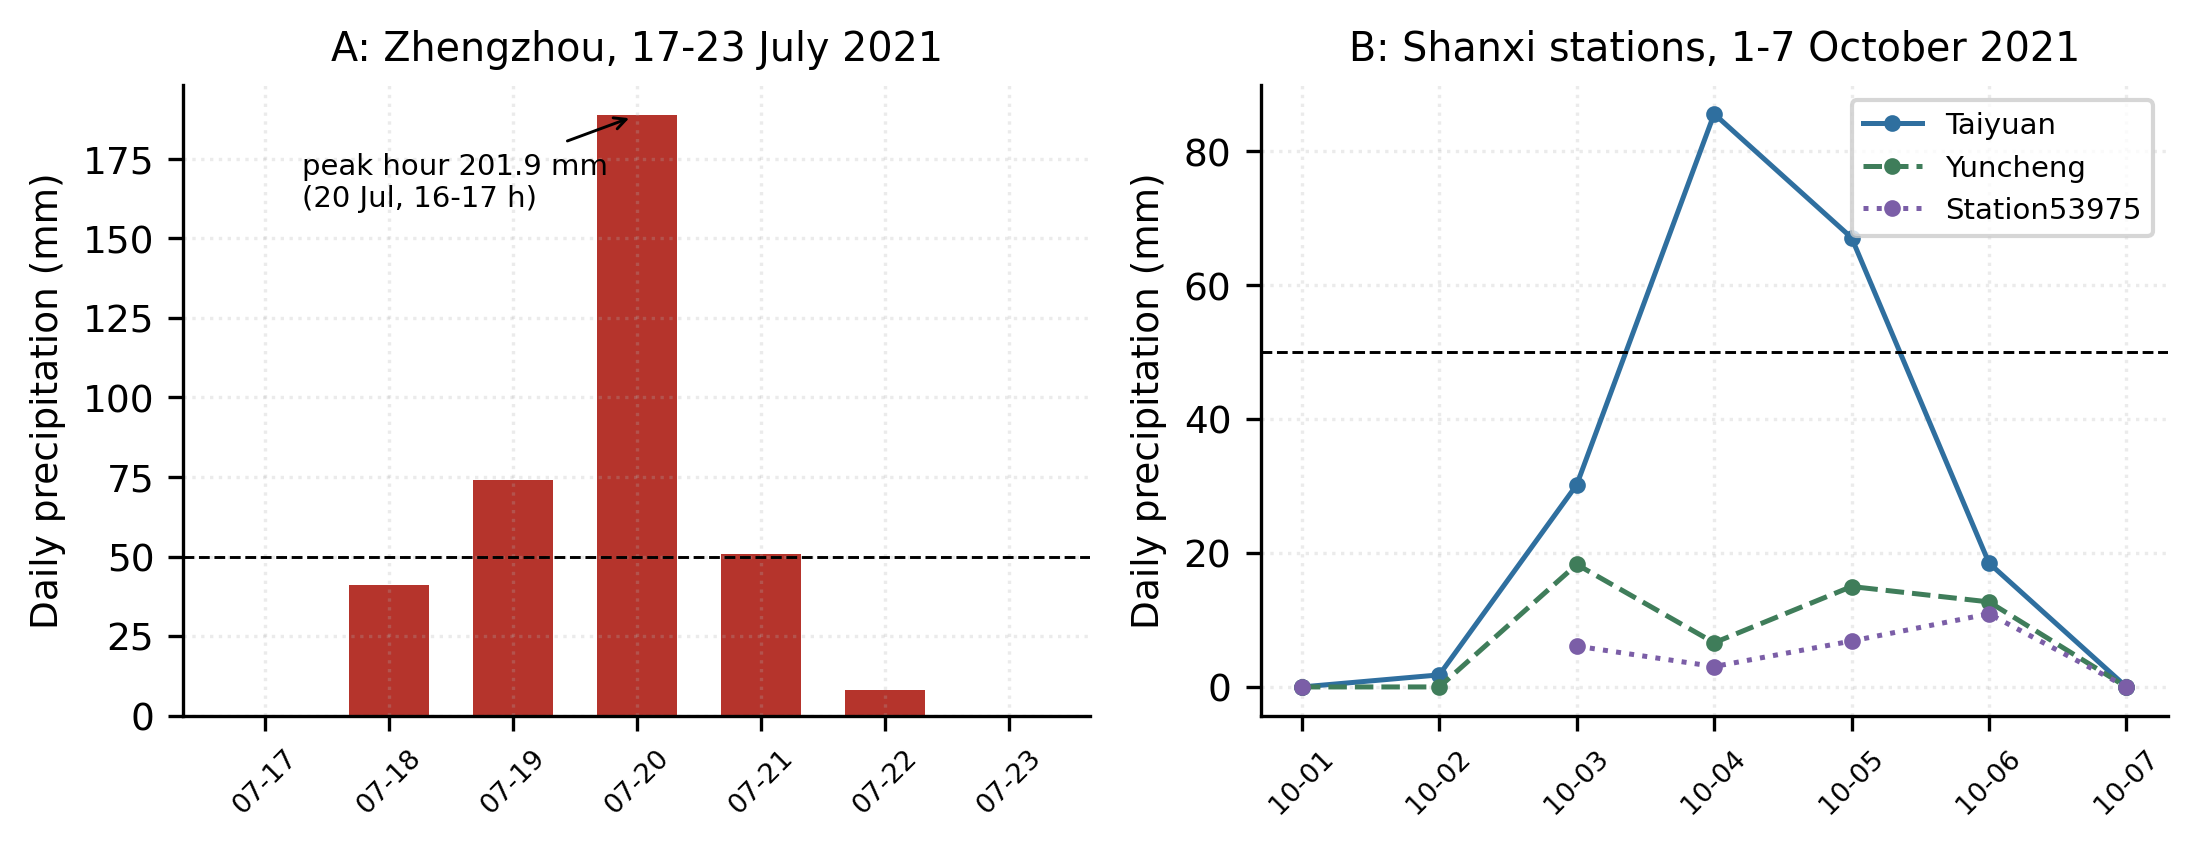
\includegraphics[width=0.38\linewidth]{../02_figures/fig16_hyetograph.png}
\caption{Daily hyetographs: (A) Zhengzhou, 17--23 July 2021, with the 201.9\,mm peak hour annotated; (B) Taiyuan, Yuncheng and station 53975, 1--7 October 2021.}
\label{fig:hyeto}
\end{figure}

\subsection{Why the losses differ by a factor of 24}

Two loss figures circulate for Henan. The problem statement quotes 655 billion CNY, a preliminary count for Zhengzhou as of 23 July 2021; the State Council investigation closed in January 2022 with 409.0 billion CNY for the municipality and 1\,200.6 billion CNY for the province \cite{sc}. We adopt the audited figures because they cover the whole event rather than its first three days, and compare provinces so that numerator and denominator come from one assessment. Table~\ref{tab:q4loss} assembles the official loss figures and normalises them. The raw ratio (23.9) is misleading because the two provinces differ in area, population and exposure. Normalising by area gives 22.4, by affected population 2.84 and by population 8.36; the raw 23.9 is the area-normalised 22.4 multiplied by the area ratio (167\,000/156\,700\,km$^2$ = 1.07). A per-millimetre ratio (6.4) is indicative only, because the two events are measured with different rainfall denominators.

\begin{table}[H]
\centering
\caption{Official losses and normalisations. Loss in $10^8$ CNY; area in km$^2$; population in millions.}
\label{tab:q4loss}
\small
\begin{tabular}{lrrr}
\toprule
 \textbf{Item} & Zhengzhou city & Henan province & Shanxi province\\
\midrule
Direct loss ($10^8$ CNY) & 409.0 & 1\,200.6 & 50.29\\
Area (km$^2$) & 7\,567 & 167\,000 & 156\,700\\
Population (millions) & 12.60 & 99.37 & 34.80\\
Affected (millions) & -- & 14.786 & 1.757\\
Deaths and missing & 380 & 398 & 18\\
\midrule
Loss per km$^2$ ($10^4$ CNY) & 540.5 & 71.9 & 3.2\\
Loss per affected (CNY) & -- & 8\,120 & 2\,862\\
Deaths per million affected & -- & 26.9 & 10.2\\
\bottomrule
\end{tabular}
\end{table}

The decomposition is an identity, not a causal test: it locates the 22-fold gap in three measurable factors rather than attributing it to rainfall. Rainfall depth explains only a factor of 2.2 (449\,mm against 203\,mm at the core stations). The remaining order of magnitude is exposure and vulnerability: Henan's plain is 2.7 times denser than Shanxi's plateau margin, the share of the provincial population affected was three times larger (14.9\% versus 5.1\%), and each affected person lost 2.8 times more, which reflects the destruction of underground space, the metro, and the fact that Zhengzhou's warning and evacuation were demonstrably too slow (the State Council report \cite{sc} documents 139 concealed deaths and a failure to suspend the metro and tunnel operations). For a planner, the lesson is that the same rainfall over a denser, more underground-dependent city produces several times the loss; reducing exposure is as effective as reducing hazard.

A multiplicative identity still leaves the question of which factor to blame, and the answer depends on the order in which the factors are switched. Averaging over all orderings settles it: with the four factors as players and their partial products as coalition worth, the Shapley value divides the 23.9-fold gap into population density $31.3\%$, affected share $33.6\%$, loss per affected person $32.7\%$ and area $2.5\%$, and the identity closes to $4\times10^{-15}$. Splitting the logarithm instead gives $31.1$, $34.1$, $32.9$ and $2.0\%$; the two conventions answer the ratio question and the level question, and neither changes the message. Single-factor removal is sharper: delete density and the gap is still $8.9$, delete the affected share $8.1$, delete severity $8.4$, delete the area ratio $22.4$. No single social factor carries the result, so the conclusion survives whichever factor a reader finds most contestable; area is irrelevant. Appendix~\ref{app:extrafig} plots the underlying normalisations (Figure~\ref{fig:lossnorm}).
